% !TEX root = ../main.tex
% Нэгдсэн хавсралт

\chapter{Хавсралт}
\label{Appendix}
\pagecolor{white}

%───────────────────────────────────────────────────────────────────────────────
\section{Судалгаанд ашигласан өгөгдлийн сангууд}

Энэхүү судалгаанд ясны хугарлын ангилал, сегментчлэл болон үнэлгээний даалгавруудад зориулан олон нийтэд нээлттэй хэд хэдэн өгөгдлийн санг ашиглав. MURA өгөгдлийг эхний хоёр туршилтын ангиллын суурь сургалтад ашигласан бол эцсийн модульчлагдсан pipeline-д бусад эх сурвалжуудыг ашигласан. Хүснэгт~\ref{tab:appA_datasets}-д ашигласан өгөгдлийн сангуудын үндсэн мэдээллийг харуулав.

\begin{table}[ht]
    \centering
    \begin{tabular}{|l|c|l|}
    \hline
    \textbf{Өгөгдлийн сан} & \textbf{Зургийн тоо} & \textbf{Даалгавар} \\ \hline
    MURA                  & $\sim$40{,}000 & Туршилт 1--2, ангиллын суурь сургалт \\ \hline
    FracAtlas             & 4{,}083  & Сегментчлэл, хугарлын зэрэг \\ \hline
    FracAtlas-COCO        & 966      & Туршилт 3-ын ангилал \\ \hline
    GRAZPEDWRI-DX         & 20{,}327 & Туршилт 3-ын ангилал \\ \hline
    YOLOBoneFracture      & 3{,}979  & Туршилт 3-ын ангилал, псевдо маск \\ \hline
    BoneFractureCVProject & 3{,}631  & Туршилт 3-ын ангилал, псевдо маск \\ \hline
    \end{tabular}
    \caption{Судалгаанд ашигласан өгөгдлийн сангууд}
    \label{tab:appA_datasets}
\end{table}

Эцсийн модульчлагдсан pipeline-д MURA-г оруулахгүйгээр нийтдээ 30{,}000 гаруй (нийлбэр $\approx$32{,}986) рентген зургийг боловсруулж ашигласан. Харин эхний хоёр туршилтын ангиллын суурь сургалтад MURA-ийн $\sim$40{,}000 зургийг тусад нь ашигласан болно.

%───────────────────────────────────────────────────────────────────────────────
\section{Хугарлын зэрэг үнэлгээний геометрийн шинж}

Хугарлын сегментчлэлийн үр дүнд үндэслэн морфологийн шинжүүдийг гарган авч хугарлын зэргийг үнэлсэн. Хүснэгт~\ref{tab:appE_geom}-д нэг жишээ тохиолдол (Grade~2)-д тооцоолсон геометрийн шинжүүдийг үзүүлэв. Хугарлын зэргийн дүрслэлийн жишээнүүдийг үндсэн үр дүнгийн бүлэгт (Бүлэг~\ref{Chapter6}) харуулсан болно.

\begin{table}[ht]
    \centering
    \begin{tabular}{|l|c|}
    \hline
    \textbf{Үзүүлэлт} & \textbf{Утга} \\ \hline
    Area (талбай, px$^2$)         & 1{,}872 \\ \hline
    Major axis (гол тэнхлэг, px)  & 55.41 \\ \hline
    Aspect Ratio (тал харьцаа)    & 1.23 \\ \hline
    Solidity (нягтрал)            & 1.00 \\ \hline
    Severity Score (зэргийн оноо) & 2 (Grade~2) \\ \hline
    \end{tabular}
    \caption{Геометрийн шинжүүдийн жишээ (Grade~2 тохиолдол)}
    \label{tab:appE_geom}
\end{table}

%───────────────────────────────────────────────────────────────────────────────
\section{Туршилтын орчин ба тохиргоо}

Туршилтуудыг гүйцэтгэхэд ашигласан техник болон програм хангамжийн орчин, сургалтын үндсэн тохиргоог дараах хүснэгтүүдэд нэгтгэн үзүүлэв.

\begin{table}[ht]
    \centering
    \begin{tabular}{|l|l|}
    \hline
    \textbf{Модуль / туршилт} & \textbf{Орчин} \\ \hline
    Туршилт 1--2 сургалт & NVIDIA RTX A6000 (48 GB) dedicated server \\ \hline
    Туршилт 3 ангилал & NVIDIA RTX A6000 (48 GB) dedicated server \\ \hline
    Туршилт 3 сегментчлэл & Google Colab, NVIDIA T4 GPU \\ \hline
    Туршилт 3 хугарлын зэрэг, эдгэрэлт & Google Colab, NVIDIA T4 GPU \\ \hline
    Нэгдсэн inference код & Google Colab, NVIDIA T4 GPU \\ \hline
    \end{tabular}
    \caption{Туршилтад ашигласан техник хангамжийн орчин}
    \label{tab:appH_hw}
\end{table}

\begin{table}[ht]
    \centering
    \begin{tabular}{|l|l|l|}
    \hline
    \textbf{Програм / сан} & \textbf{Хувилбар} & \textbf{Зориулалт} \\ \hline
    Python                       & 3.10            & Үндсэн програмчлалын хэл \\ \hline
    PyTorch (torch)              & 2.1 (cu121)     & Гүн сургалтын фреймворк \\ \hline
    torchvision                  & 0.16            & Дүрсний хувиргалт, загвар \\ \hline
    CUDA                         & 12.1            & GPU тооцоолол \\ \hline
    timm                         & 1.0             & ConvNeXt, EfficientNet backbone \\ \hline
    segmentation-models-pytorch  & 0.3             & ResNet50 U-Net сегментчлэл \\ \hline
    Segment Anything (SAM)       & ViT-B           & Псевдо маск үүсгэх \\ \hline
    albumentations               & 1.4             & Өгөгдөл нэмэгдүүлэлт \\ \hline
    OpenCV (opencv-python)       & 4.9             & Дүрс боловсруулалт \\ \hline
    NumPy                        & 1.26            & Тоон тооцоолол \\ \hline
    Pandas                       & 2.2             & Өгөгдөл боловсруулалт \\ \hline
    scikit-learn                 & 1.4             & Random Forest (хугарлын зэрэг) \\ \hline
    scikit-image                 & 0.22            & Морфологийн шинж тооцоолол \\ \hline
    SciPy                        & 1.11            & Шинжлэх ухааны тооцоолол \\ \hline
    pytorch-grad-cam             & 1.5             & Grad-CAM тайлбарлалт \\ \hline
    SHAP                         & 0.44            & SHAP тайлбарлалт \\ \hline
    Matplotlib                   & 3.8             & График дүрслэл \\ \hline
    \end{tabular}
    \caption{Програм хангамж}
    \label{tab:appH_sw}
\end{table}

\begin{table}[ht]
    \centering
    \begin{tabular}{|l|l|}
    \hline
    \textbf{Үзүүлэлт} & \textbf{Утга} \\ \hline
    Batch Size    & 16 \\ \hline
    Epochs        & 50 (10 хөлдөөсөн + 40 бүрэн) \\ \hline
    Optimizer     & AdamW \\ \hline
    Learning Rate & $1\times10^{-4}$ \\ \hline
    Image Size    & $512\times512$ \\ \hline
    Random Seed   & 42 \\ \hline
    \end{tabular}
    \caption{Сургалтын үндсэн тохиргоо}
    \label{tab:appH_train}
\end{table}

%───────────────────────────────────────────────────────────────────────────────
\section{Судалгааны кодын GitHub репозитор}

Судалгааны ажлын эх код, туршилтын сургалт болон inference хийхэд ашигласан script, notebook, мөн дипломын тайлангийн \LaTeX{} эх файлуудыг GitHub репозиторт байршуулсан. Репозиторийн холбоос: \href{https://github.com/Ariuntungalag23/diploma}{\texttt{github.com/Ariuntungalag23/diploma}}.

Репозиторт ангилал, сегментчлэл, хугарлын зэрэг болон эдгэрэлтийн төлөвийг үнэлэх proof-of-concept модулиудын код, туршилтын туслах script-үүд, тайлангийн эх материалууд багтсан. Харин өгөгдлийн сан, сургасан model weight, checkpoint, завсрын үр дүнгийн том хэмжээтэй файл болон хувийн тохиргооны файлуудыг хэмжээ, лиценз, нууцлалын шалтгаанаар оруулаагүй. Эдгээр файлыг репозиторийн \texttt{.gitignore} тохиргоогоор тусгаарласан бөгөөд өгөгдлийг тухайн олон нийтэд нээлттэй эх сурвалжаас тусад нь татаж ашиглах шаардлагатай.

Эцсийн хувилбарыг GitHub-д \texttt{diploma\_ariuntungalag} commit нэрээр байршуулсан. Энэ нь судалгаанд ашигласан кодын бүтцийг шалгах, туршилтын pipeline-ийг давтан ажиллуулах болон тайлангийн эхийг хянах боломжийг бүрдүүлнэ.

%───────────────────────────────────────────────────────────────────────────────
\section{Хиймэл оюуны хэрэгслийн ашиглалт}

Энэхүү судалгааны ажлын явцад хиймэл оюуны хэрэгслүүдийг зөвхөн туслах зориулалтаар ашигласан.

\begin{table}[ht]
    \centering
    \begin{tabular}{|l|l|}
    \hline
    \textbf{Хэрэгсэл} & \textbf{Ашигласан зориулалт} \\ \hline
    ChatGPT        & Бичвэрийн найруулга, хэл зүй болон үг үсгийн алдаа шалгах \\ \hline
    GitHub Copilot & Кодын автомат гүйцээлт, алдаа засахад туслах \\ \hline
    \end{tabular}
    \caption{AI хэрэгслийн ашиглалт}
    \label{tab:appI_ai}
\end{table}

Хиймэл оюуны хэрэгслүүдийг судалгааны үр дүн, туршилтын хэмжилт, статистик тооцоолол болон эцсийн дүгнэлтийг автоматаар үүсгэхэд ашиглаагүй болно. Судалгааны бүх туршилт, өгөгдөл боловсруулалт, үр дүнгийн үнэлгээ болон шинжилгээг судлаач өөрөө гүйцэтгэсэн болно.

%───────────────────────────────────────────────────────────────────────────────
\section{Нэмэлт зураг}

Энэ хэсэгт үндсэн бүлгийн хэлэлцүүлгийг нэмж тодотгох зорилгоор сегментчлэлийн нэмэлт жишээ, нэгдсэн pipeline-ийн жишээ дүгнэлт болон модуль хоорондын зөрчлийн нэмэлт жишээг үзүүлэв.

\begin{figure}[H]
    \centering
    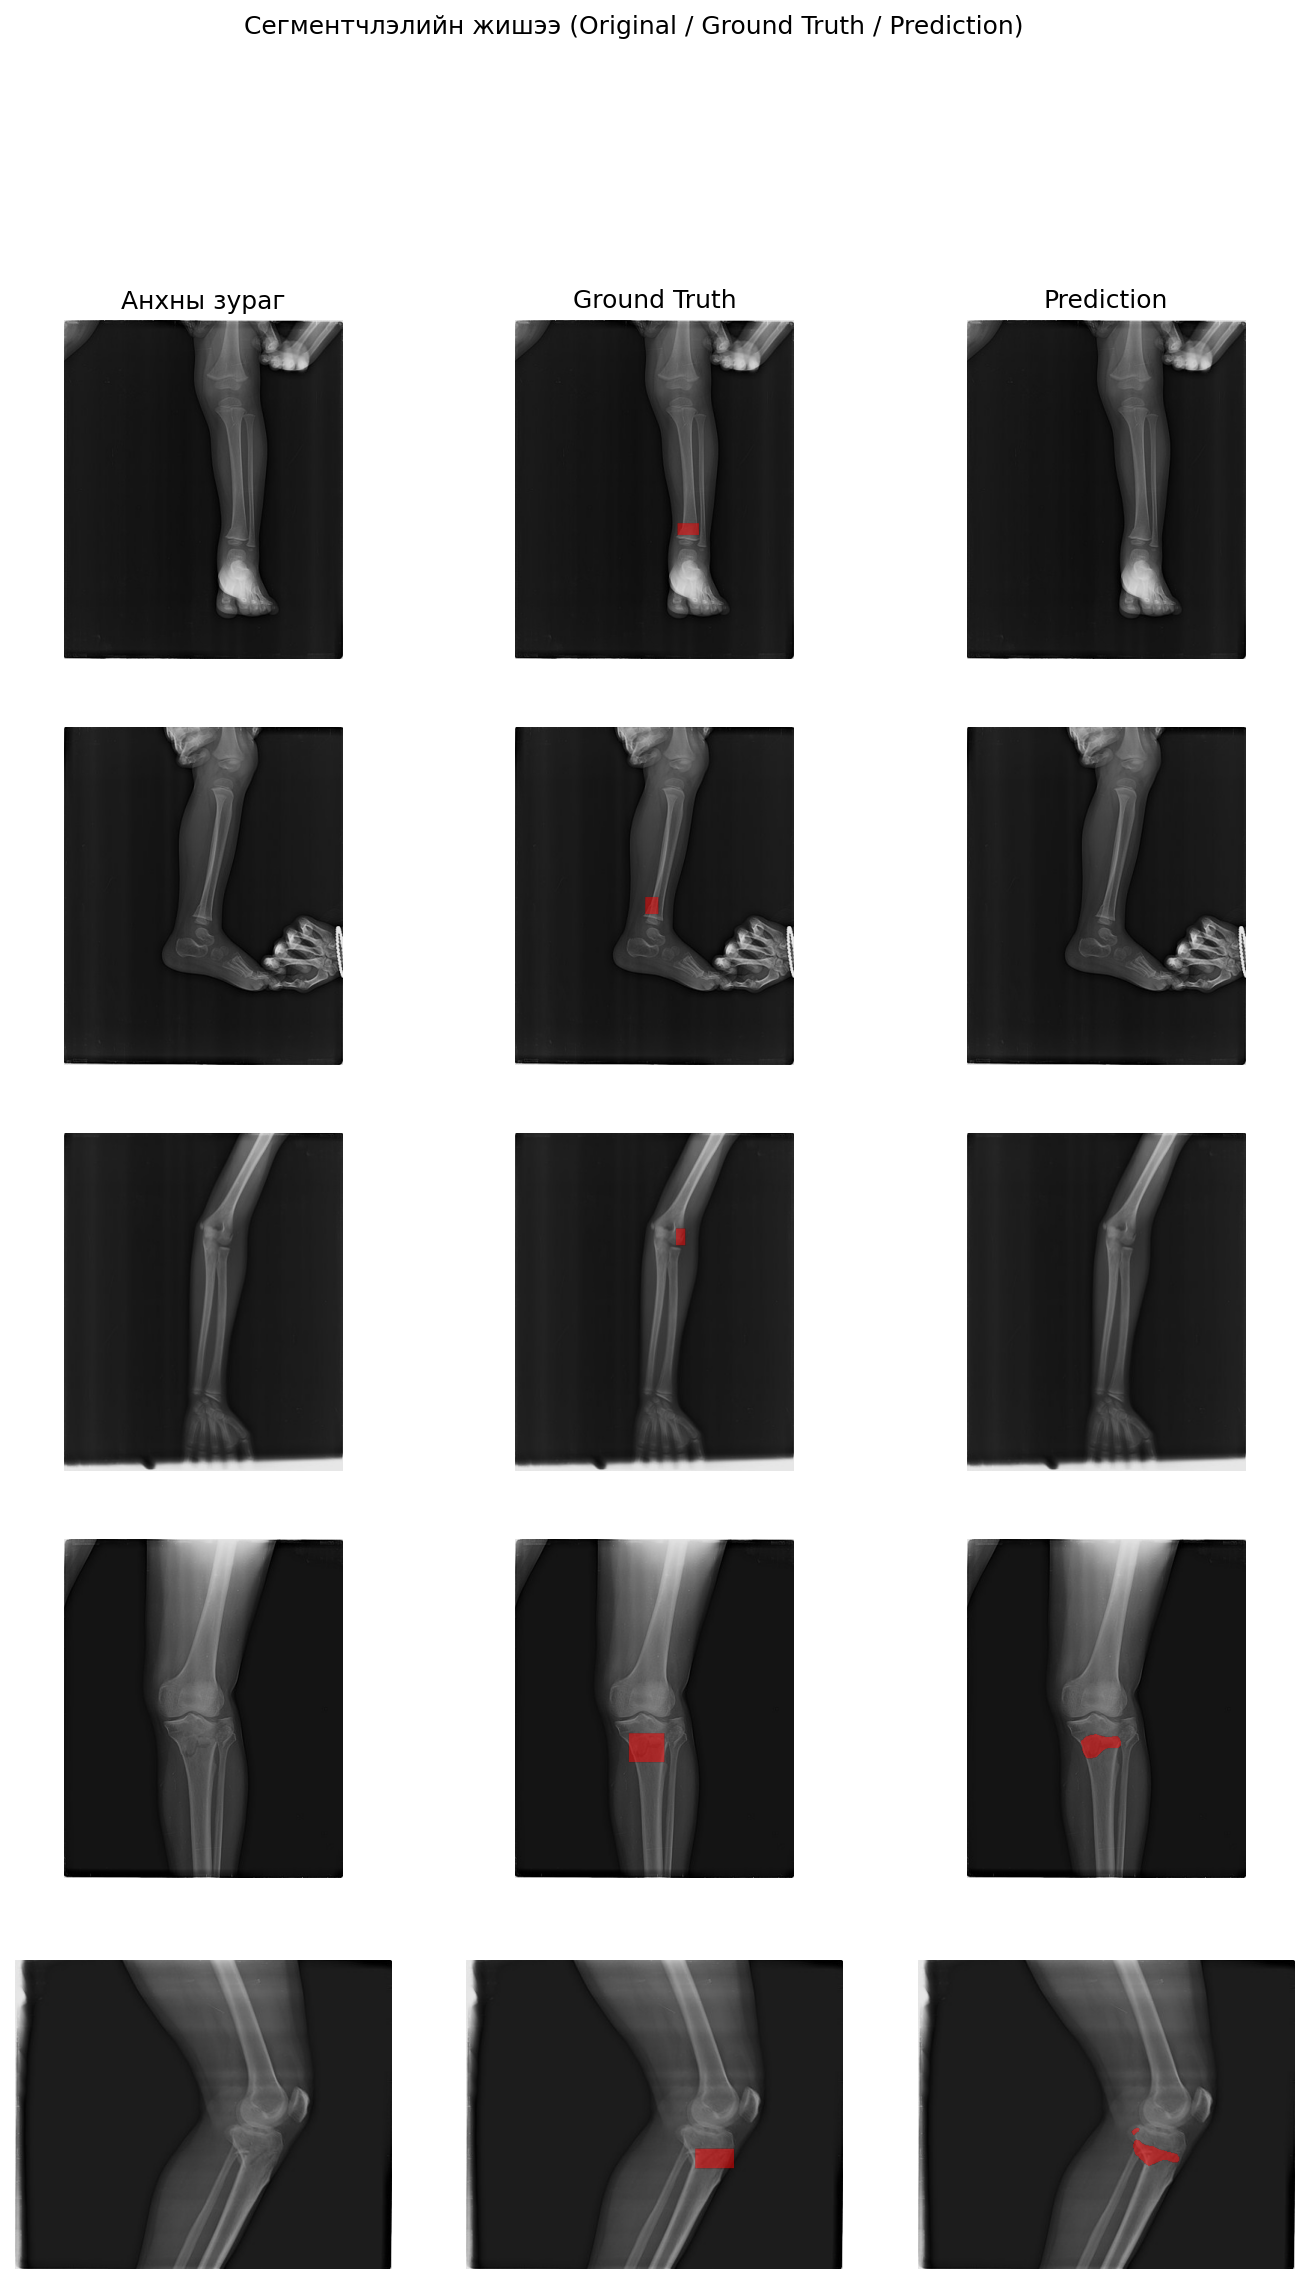
\includegraphics[width=\textwidth,height=0.85\textheight,keepaspectratio]{Figures/appx_d3_seg_triplets.png}
    \figcaption{Нэмэлт сегментчлэлийн жишээнүүд}{Нэмэлт сегментчлэлийн жишээнүүд — анхны рентген зураг, лавлах маск (GT) болон загварын таамагласан маскийн харьцуулалт}
    \label{fig:seg_more}
\end{figure}

\begin{figure}[H]
    \centering
    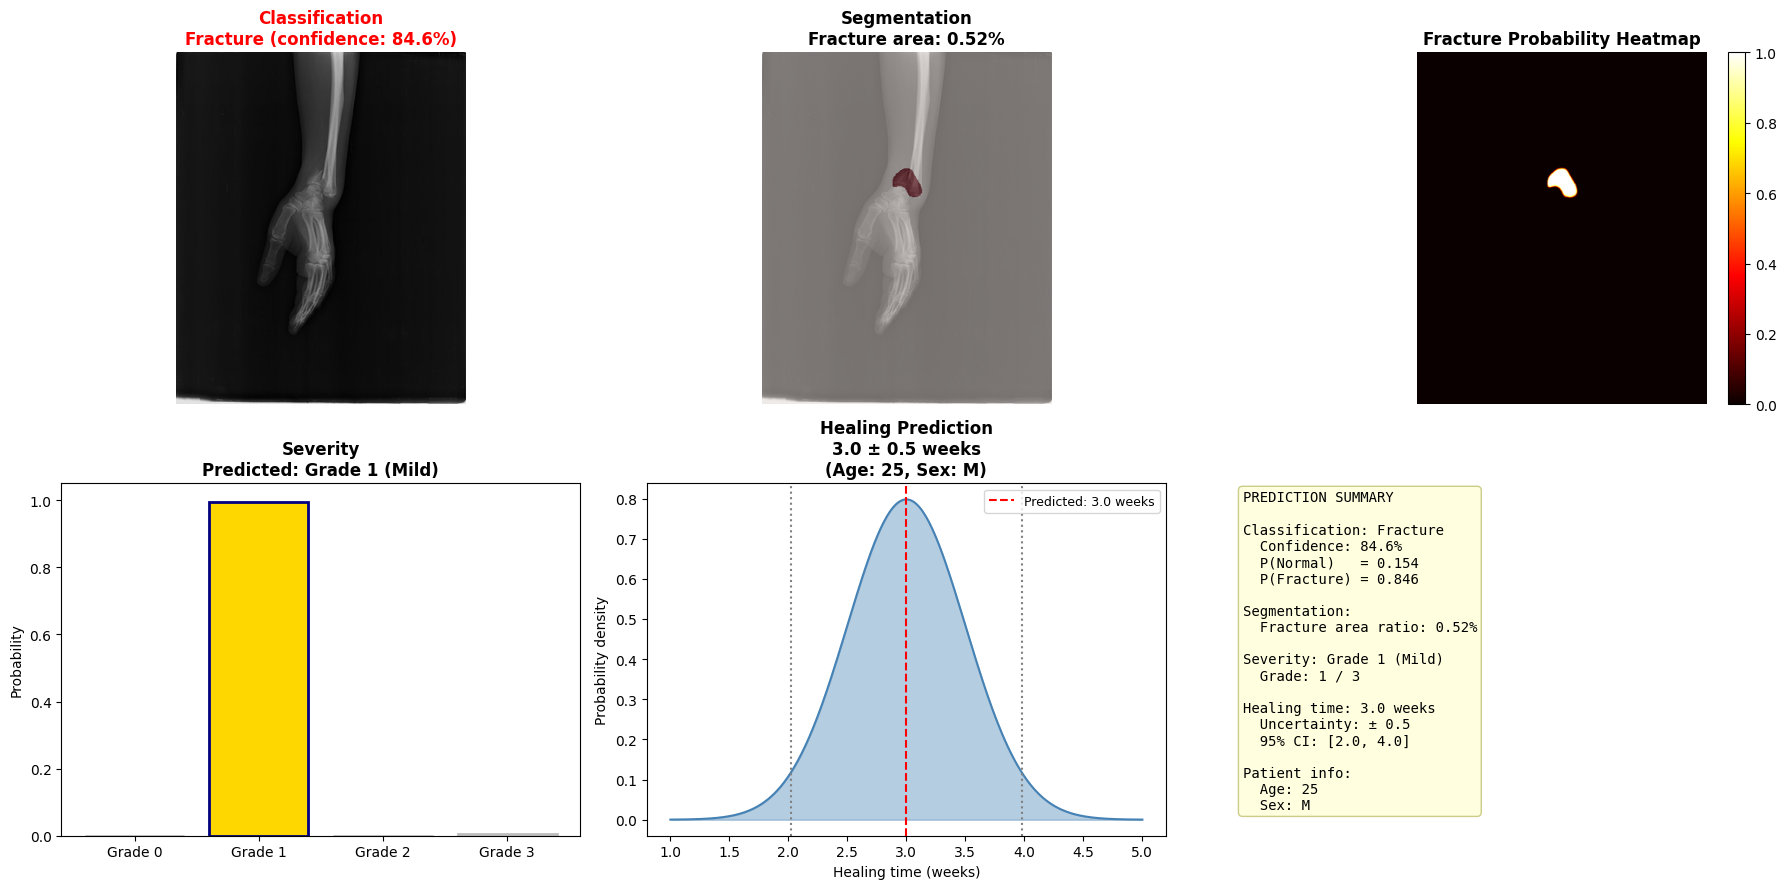
\includegraphics[width=\textwidth]{Figures/t3_predict_example.png}
    \figcaption{Бугуйн хугарлын жишээ таамаглал}{Бугуйн хугарлын жишээ таамаглал: ангилал \emph{Fracture} (итгэл 84.6\%), Grade~1 (Mild), эдгэрэлт $\approx$3 долоо хоног}
    \label{fig:pred_wrist}
\end{figure}

\begin{figure}[H]
    \centering
    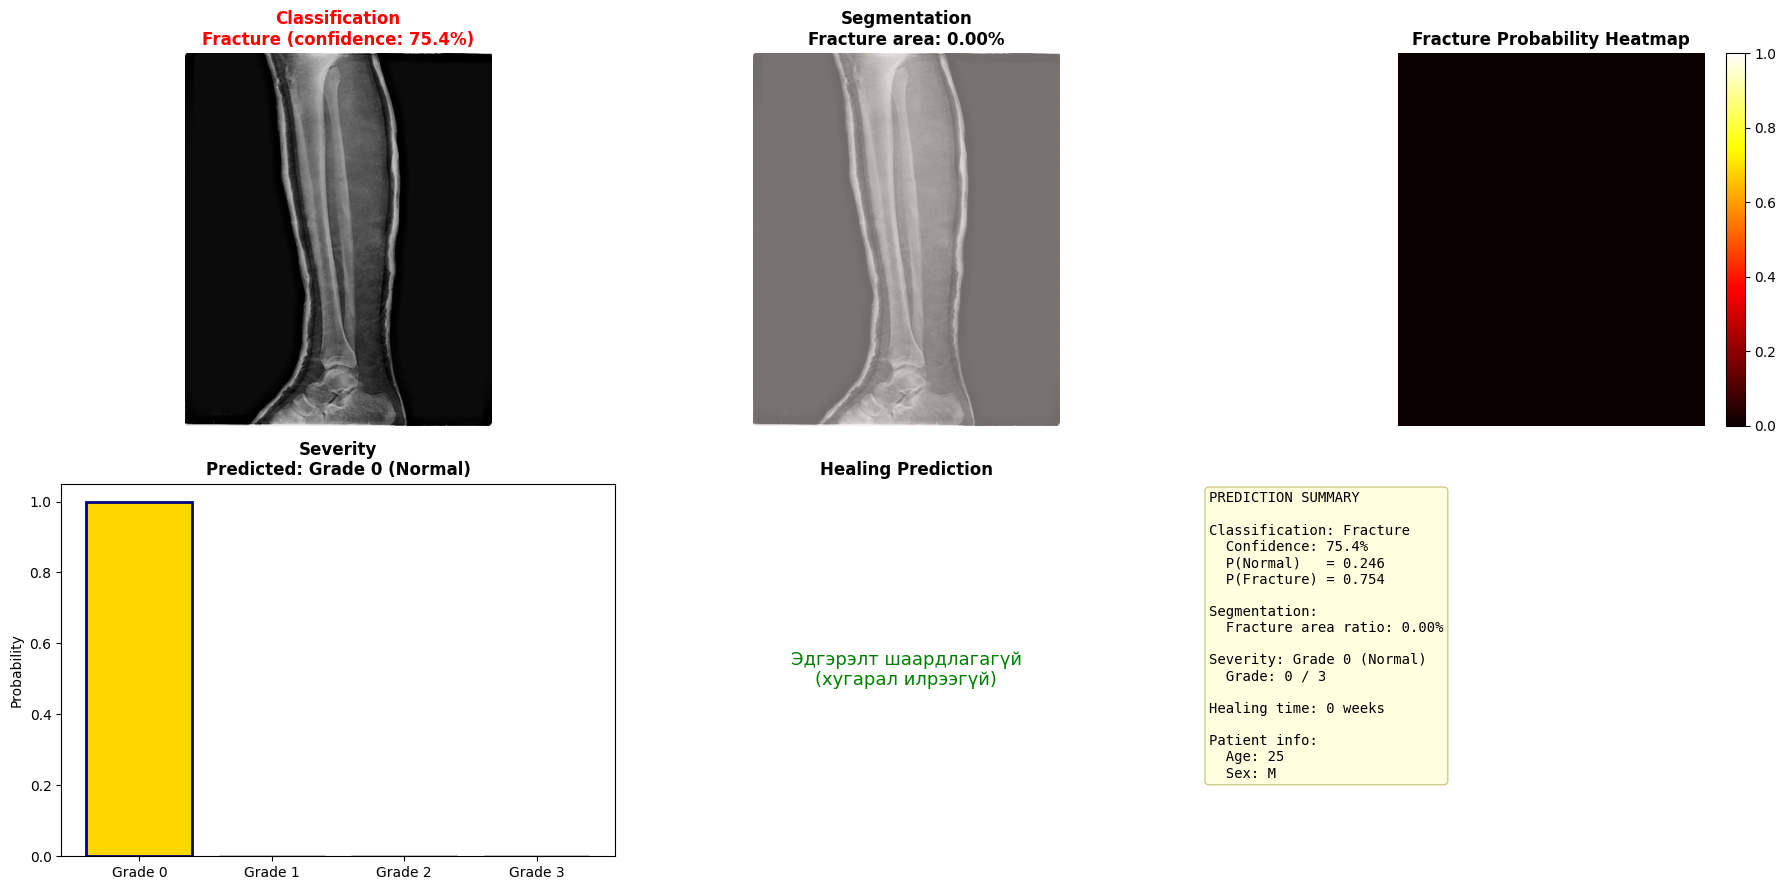
\includegraphics[width=\textwidth]{Figures/t3_pred_demo_9.png}
    \figcaption{Модуль хоорондын зөрчлийн жишээ 2}{Модуль хоорондын зөрчлийн өөр жишээ (IMG0003704): $P=0.754$ боловч маск гараагүй}
    \label{fig:err_disagree2}
\end{figure}
